\documentclass[a4paper, 11pt]{article}
\usepackage[polish]{babel}
\usepackage[MeX]{polski}
\usepackage[utf8]{inputenc}
\usepackage[T1]{fontenc}
%\usepackage{times}
\usepackage{graphicx,wrapfig}
%\usepackage{anysize}
%\usepackage{tikz}
%\usetikzlibrary{calc,through,backgrounds,positioning}
\usepackage{anysize}
\usepackage{float}
%\usepackage{stmaryrd}
%\usepackage{amssymb}
%\usepackage{amsthm}
%\marginsize{3cm}{3cm}{3cm}{3cm}
%\usepackage{amsmath}
%\usepackage{color}
%\usepackage{listings}
%\usepackage{enumerate}
%\lstloadlanguages{Ada,C++}


\begin{document}	
	% \noindent -  w tym akapicie nie bedzie wciecia
	% \ indent - to jest aut., ale powoduje ze jest wciecie
	% \begin{flushleft}, flushright, center - wyrownianie akapitu
	% \textbf{pogrubiany tekst}
	% \textit{kursywa} 
	% 					STRONY 
	%  http://www.codecogs.com/latex/eqneditor.php 
	%  http://www.matematyka.pl/latex.htm
	% 
	\begin{titlepage}
		
		
		
		\newcommand{\HRule}{\rule{\linewidth}{0.5mm}} % Defines a new command for the horizontal lines, change thickness here
		
		\center % Center everything on the page
		
		%----------------------------------------------------------------------------------------
		%	HEADING SECTIONS
		%----------------------------------------------------------------------------------------
		
		\textsc{\LARGE Akademia Górniczo-Hutnicza im. Stanisława Staszica}\\[1.5cm] % Name of your university/college
		\textsc{\Large Kraków}\\[0.5cm] % Major heading such as course name
		\textsc{\large }\\[0.5cm] % Minor heading such as course title
		
		%----------------------------------------------------------------------------------------
		%	TITLE SECTION
		%----------------------------------------------------------------------------------------
		
		\HRule \\[0.4cm]
		{\fontsize{38}{50}\selectfont Osadnicy z Catan - Gra sieciowa}
		%	{ \Huge \bfseries} Osadnicy z Catan - Gra sieciowa\\[0.3cm] % Title of your document
		\HRule \\[1.5cm]
		
		%----------------------------------------------------------------------------------------
		%	AUTHOR SECTION
		%----------------------------------------------------------------------------------------
		
		% If you don't want a supervisor, uncomment the two lines below and remove the section above
		\Large \emph{Autorzy:}\\
		Marcin \textsc{Jędrzejczyk}\\ % Your name
		Sebastian \textsc{Katszer}\\ % Your name
		Katarzyna \textsc{Kosiak} \\
		Paweł \textsc{Ogorzały}\\[3cm]\ % Your name
		
		
		%----------------------------------------------------------------------------------------
		%	DATE SECTION
		%----------------------------------------------------------------------------------------
		
		{\large \today}\\[3cm] % Date, change the \today to a set date if you want to be precise
		
		%----------------------------------------------------------------------------------------
		%	LOGO SECTION
		%----------------------------------------------------------------------------------------
		
		%\includegraphics{Logo}\\[1cm] % Include a department/university logo - this will require the graphicx package
		
		%----------------------------------------------------------------------------------------
		
		\vfill % Fill the rest of the page with whitespace
		
	\end{titlepage}
	
	%SPIS TRESI
	%
	%
	%
	%
	%
	%
	%
	%
	%
	
	\tableofcontents
	\vfill
	\newpage	%\pagebreak
	
	%SEKCJE
	%opis zagadnienia, temat, problem, dlaczego chcemy to rozwiązacyać metodą ewolucyjnę
	%jakie są metody rozwiącania problemu, przegląd literatury,
	%proponowane rozwiązania (spójność)
	%czym się inspierowałyśmy
	%
	%
	%
	
	%\setlength{\parskip}{1ex plus 0.5ex minus 0.2ex}
	
	\section{Wstęp}
	\indent
	
	Niniejszy dokument stanowi dokumentację projektu ``Osadnicy z Catanu - Gra sieciowa'' z przedmiotu Wprowadzenie do Wzorców Projektowych.
	Nasz projekt zrealizowaliśmy
	\subsection{Dlaczego Catan?}
	\indent 
	
	Nasza grupa projektowa składa się z osób zafascynowanych światem zarówno gier planszowych jak i komputerowych. Projekt ten umożliwia nam połączenie naszych zainteresowań. Wybór padł na grę ``Osadnicy z Catanu'' z bardzo prostego powodu: dzięki prostocie i przejrzystości zasad stanowi ona idealny start dla osób, które chcą rozpocząć swoją przygodę z grami planszowymi. \\ 
	
	Dzięki wprowadzeniu rozgrywki sieciowej możliwe jest rozegranie partii z przyjaciółmi z całego świata bez dodatkowych wydatków, a także rozpowszechnienie tej gry i ułatwienie wejścia w świat gier planszowych. 
	\subsection{Opis gry}
	\indent
	
	Osadnicy z Catanu (Settlers of Catan) to jedna z najpopularniejszych rodzinno-ekonomicznych gier planszowych na świecie. 
	%do cytatu
	Gracze są osadnikami na niedawno odkrytej wyspie Catan. Każdy z nich przewodzi świeżo założonej kolonii i rozbudowuje ją stawiając na dostępnych obszarach nowe drogi i miasta. Każda kolonia zbiera dostępne dobra naturalne, które są niezbędne do rozbudowy osiedli.
	
	Gracz musi rozważnie stawiać nowe osiedla i drogi, aby zapewnić sobie dostateczny, ale zrównoważony dopływ zasobów, a jeśli ma ich nadmiar - prowadzić handel z innymi graczami sprzedając im owce, drewno, cegły, zboże lub żelazo a pozyskując od nich te zasoby, których ciągle mu brakuje.
	
	Pierwszy z graczy, który uzyska 10 punktów z wybudowanych przez siebie dróg, osiedli i specjalnych kart - wygrywa.
	
	%skrócone zasady	
	
	%	automaty gdzies!!!!!!\\
	
	
	
	
	
	\section{Użyte wzorce projektowe}
	\subsection{Singleton}
	\indent
	
	Singleton jest kreacyjnym wzorcem projektowym, którego zadaniem jest ograniczenie możliwości tworzenia obiektów danej klasy do jednej instancji, oraz zapewnienie globalnego dostępu do stworzonego obiektu.
	
	Singleton implementuje się poprzez stworzenie klasy, która posiada statyczną metodę, która sprawdza czy istnieje instancja danej klasy, w razie potrzeby tworząc ją. Następnie instancja zwracana jest przez referencję. Aby uniemożliwić tworzenie dodatkowych instancji, konstruktor klasy deklaruje się jako prywatny lub chroniony.
	
	Wzorzec ten ma u nas zastosowanie w przypadku klas odpowiadajacych za kostkę, planszę. Zapewnia on globalny dostęp oraz ogranicza możliwość tworzenia większej liczby instancji. 
	
	\subsection{Builder}
	\indent
	
	Builder jest wzorcem konstrukcyjnym, który ma za zadanie oddzielenie tworzenia obiektów od ich reprezentacji. 
	Proces tworzenia obiektu podzielony jest na mniejsze etapy, a każdy z nich może być implementowany na wiele różnych sposobów. Umożliwia to tworzenie różnych reprezentacji obiektów w tym samym procesie konstrukcyjnym.
	Konstruowanie obiektu następuje poprzez wcześniejsze stworzenie jego fragmentów.
	
	
	Na wzorzec składa się:
	\begin{itemize}
		
		\item Builder - dostarcza inferfejs do tworzenia obiektów nazywanych produktami,
		\item ConcreteBuilder - tworzy konkretne reprezentacje produktów przy pomocy zaimplementowanego interfejsu Builder,
		\item Director - zleca konstrukcję produktów poprzez obiekt Builder.
	\end{itemize}
	
	W naszym projekcie wzorzec ten znajduje zastosowanie przy tworzeniu planszy, która składa się z kafli.
	
	
	\subsection{Abstract Factory}
	\indent
	
	Kreacyjny wzorzec projektowy, który pozwala tworzyć całe rodziny produktów. Dostarcza on interfejs do tworzenia różnych obiektów jednego typu bez specyfikowania ich konkretnych klas.
	
	Wzorzec ten wykorzysytwany będzie przy konstruowaniu kafli oraz generowaniu kart.
	
	
	\subsection{Observer}
	Wzorzec "Observer" jest używany jeśli występuje relacja jeden do wielu pomiędzy obiektami. Modyfikacja jednego obiektu powoduje, że zależne obiekty są powiadamiane automatycznie. Wzorzec ten podchodzi pod kategorię wzorców czynnościowych.\\
	%Observer pattern is used when there is one-to-many relationship between objects such as if one object is modified, its depenedent objects are to be notified automatically. Observer pattern falls under behavioral pattern category.\\
	%	"That’s what the observer pattern is for. It lets one piece of code announce that something interesting happened without actually caring who receives the notification."\\
	%	komunikacja\\
	Wzorzec ten pomoże nam w komunikacji między graczami. Będziemy wysyłać informacje o tym co się zmieniło na planszy. A OBSERVER każdego gracza będzie je wyłapywał i egzekwował.
	\subsection{State}
	\indent
	We wzorcy "State" zachowanie klasy zmienia się w zalezności od jej stanu. Ten typ wzorca wchodzi pod wzorce czynnościowe.\\
	%	In State pattern a class behavior changes based on its state. This type of design pattern comes under behavior pattern.
	Tworzymy obiekty, które reprezentują różne stany i konteksty obiektu, którego zachowanie zmienia się tak jak jego stan.
	%%In State pattern, we create objects which represent various states and a context object whose behavior varies as its state object changes.\\
	W zależności od tego jaką kartę zagramy stan planszy może się zmienić. Możemy wybudować drogi, wejść w interakcję z innymi graczami, czy zablokować dochód z danego pola. Dlatego potrzebujemy wzorca odpowiedzialnego za zajmowanie się stanem klasy.
	%złodziej,karty specjalne, drogi\\
	\subsection{Command}
	
	%Command pattern is a data driven design pattern and falls under behavioral pattern category. A request is wrapped under an object as command and passed to invoker object. Invoker object looks for the appropriate object which can handle this command and passes the command to the corresponding object which executes the command.
	Wzorzec "Command" opakowuje żądania w obiekty jako rozkaz i przesyła do obiektu wzywającego (z ang. invoker). Obiekt wzywający szuka obiektu właściwego, który może zająć się tym rozkazem i   przesyła rozkaz do odpowiedniego obiektu który wykonuje rozkaz.\\  
	Wzorzec ten należy do wzorców czynnościowych, czyli opisujących sposób przepływu danych w złożonych aplikacjach.%to z Polskiej strony mam
	??? Skorzystamy z niego, by móc zagrywać karty rozwoju, które są swoistymi rozkazami. Wzorzec ten będzie musiał u nas współpracować z kodem napisanym pod wzorzec "State". %??? co wy na to
	TO DO gdzie z tego skorzystamy
	Commands are an object-oriented replacement for callbacks.\\
	\section{Użyte biblioteki zewnętrzne}
	\subsection{Biblioteka graficzna}
	\indent
	
	Jeśli chodzi o bibliotekę graficzną, to nasz wybór padł na libGDX - crossplatformową bibliotekę z licencją opensource (oficjalna strona internetowa: www.libgdx.badlogicgames.com). 
	
	Jedną z głównych zalet tej biblioteki jest jej szybkość - twórcy postawili bardzo duży nacisk na rozsądne zarządzanie pamięcią.  Dodatkowo libGDX dostarcza narzędzi do obsługi dźwięku i interpretacji wejścia dostarczonego przez użytkownika. Mimo, że renderowanie zachodzi przy użyciu OpenGL ES 2.0, to w większości przypadków nie trzeba znać szczegółów działania tego API, ponieważ biblioteka libGDX dostarcza wygodnych, wysokopoziomowych metod, dzięki którym sprawnie można uzyskać pożądane efekty - od wyświetlania dwuwymiarowych obiektów po tworzenie trójwymiarowych scen.
	

	\subsection{Biblioteka sieciowa}
	\indent
	
	Jako architekturę do połączeń internetowych wybraliśmy Peer-2-Peer. Powodem jest brak zewnętrznego serwera jak i chęć nauczenia się nowych technologii. Do jej implementacji wykorzystana zostanie biblioteka JXTA, która rozpowszechniona jest na licencji opensource. JXTA jest zbiorem sześciu protokołów, za pomocą których jesteśmy w stanie połączyć się z innymi węzłami w sieci, nawet jeśli znajdują się one za NAT-em czy też za Firewallem. Jest on niezależny od systemu operacyjnego, języka programowania, wykorzystywanego protokołu transportowego oraz jest dla każdego urządzenia cyfrowego. 
	
	Nawiązanie połączenia pomiędzy węzłami jest możliwe dzięki peer groups.  Dla każdej grupy urządzeń tworzona jest grupa, sieć wirtualna, która jest niezależna od rzeczywistej topologii, w ramach której udostępniane są usługi i następuje wymiana danych. Utworzenie tej grupy jak i jej znalezienie przez innych użytkowników jest możliwe dzięki advertisment, która jest swoistą wizytówką. Każdy korzystający z JXTA znajduje się domyślnie w światowej grupie, w której może wyszukać czy też propagować grupę. Wszystkie informacje są przekazywane za pomocą pipe-ów, które dzielą się na wejściowe i wyjściowe. Umożliwiają one komunikację typu jeden do jeden, jeden do wielu, wielu do wielu.
	
		
	\section{Architektura}
	\indent
	
	Poniżej prezentujemy opis wszystkich warstw, na które podzieliliśmy naszą aplikację.
	%screen z głównym uml
	\begin{figure}[H]%[!htb]
		\includegraphics[scale=0.5]{uml/main.jpg}\caption{Podział na warstwy}
	\end{figure}
	
	\subsection{Warstwa prezentacji}	
	\begin{figure}[H]%[!htb]
		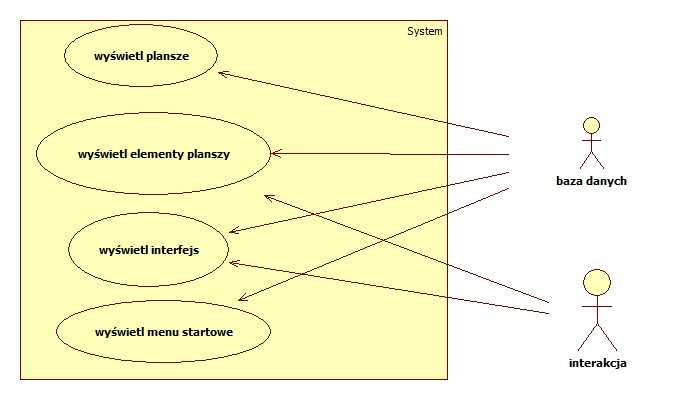
\includegraphics[scale=0.5]{uml/UseCasePrezentacja.jpg}
	\end{figure}
	\subsection{Warstwa interakcji}
	\begin{figure}[H]%[!htb]
		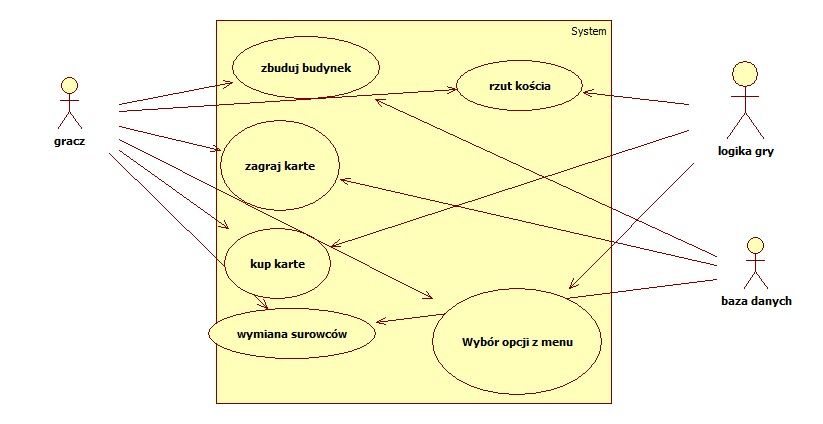
\includegraphics[scale=0.5]{uml/UseCaseInterakcja.jpg}
	\end{figure}	
	\subsection{Warstwa logiki gry}	
	\begin{figure}[H]%[!htb]
		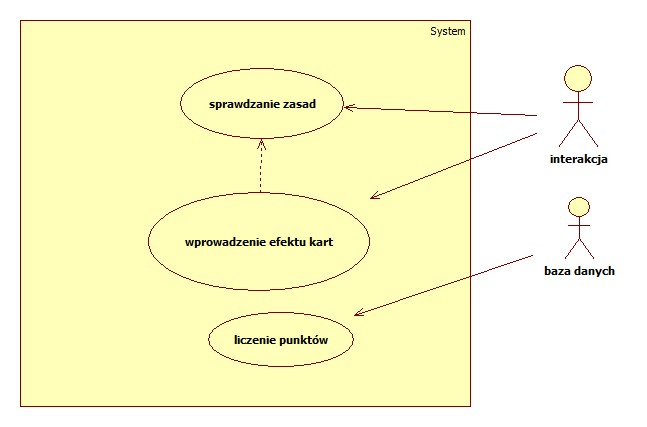
\includegraphics[scale=0.5]{uml/UseCaseLogikaGry.jpg}
	\end{figure}
	\subsection{Warstwa baz danych}	
	\begin{figure}[H]%[!htb]
		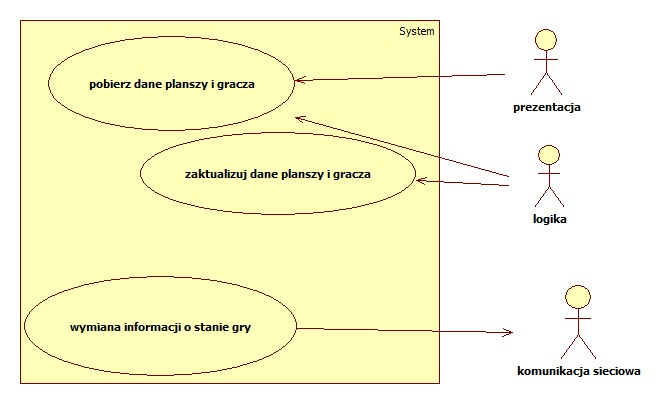
\includegraphics[scale=0.5]{uml/UseCaseBazaDanych.jpg}
	\end{figure}
	\subsection{Warstwa komunikacji sieciowej}
	\begin{figure}[H]%[!htb]
		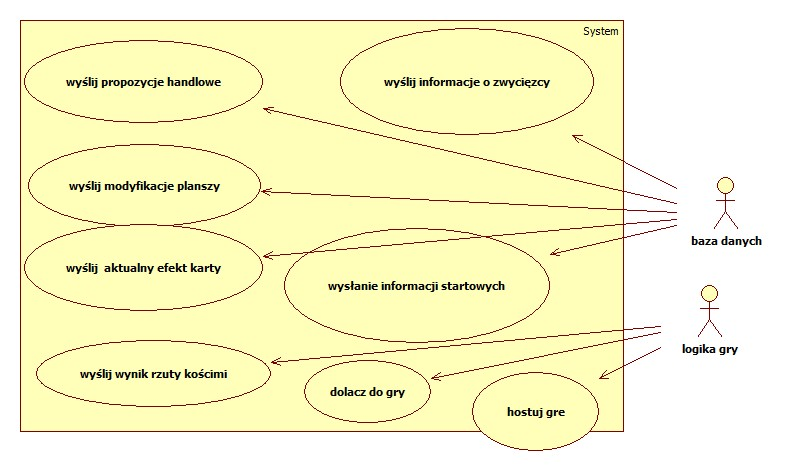
\includegraphics[scale=0.5]{uml/UseCaseKomunikacja.jpg}
	\end{figure}	
	
	
	
	\section{Podsumowanie}
	
	
	\section{Testy}
	
	
	\section{Wnioski}
	
	
	\section{Literatura}
	
	\textbf{Asensio MI, Ferragut L., Simon J.:} Modelling of convective phenomena in forest fire. Rev Real Academia de Ciencias, 2002, 96:299–313\\
	
	
\end{document}
